\documentclass{article}
\usepackage{amsmath}
\usepackage{amssymb}
\usepackage{indentfirst}
\usepackage{graphicx}
\usepackage{color}
\usepackage{fancyhdr}
\usepackage{epstopdf}
\usepackage{indentfirst}
\usepackage{geometry}
\geometry{left=2.5cm,right=2.5cm,top=2.5cm,bottom=2.5cm}

\title{14.03 Problem Set 1}
\author{Yijun Jiang}
%\email{yjjiang@mit.edu}
\date{\today}

\pagestyle{fancy}
\lhead{Yijun Jiang}
\rhead{14.03 Problem Set 1}

\begin{document}
\maketitle
\section{Implicit Function Theorem and Envelop Theorem}
\subsection{Subproblem 1}
\begin{align*}
	\frac{\partial y}{\partial x}&=4a-14x=0\\
	x&=x^*(a)=\frac{2}{7}a
\end{align*}

\subsection{Subproblem 2}
\begin{equation*}
	\frac{\partial^2y}{\partial^2x}=-14<0
\end{equation*}

Therefore, $x^*(a)$ is a maximum.

\subsection{Subproblem 3}
\begin{equation*}
	y^*(a)=4ax^*(a)-7x^*(a)^2=\frac{4}{7}a^2
\end{equation*}

\subsection{Subproblem 4}
\begin{align*}
	\frac{dx^*(a)}{da}&=\frac{d}{da}\left(\frac{2}{7}a\right)=\frac{2}{7}\\
	\frac{dy^*(a)}{da}&=\frac{d}{da}\left(\frac{4}{7}a^2\right)=\frac{8}{7}a
\end{align*}

\subsection{Subproblem 5}
The FOC in (1) reads
\begin{equation*}
	g(x^*;a)=4a-14x^*=0
\end{equation*}

Therefore, according to implicit function theorem,

\begin{equation*}
	\frac{dx^*}{da}=-\frac{\partial g/\partial a}{\partial g/\partial x^*}=\frac{2}{7}
\end{equation*}

This agrees with direct calculation from the expression of $x^*(a)$.

\subsection{Subproblem 6}
According to the envelope theorem,
\begin{equation*}
	\frac{d^*y(a)}{da}=\left.\frac{\partial y}{\partial a}\right|_{x=x^*(a)} =4x^*(a)=\frac{8}{7}a
\end{equation*}

This theorem simplifies the calculation in that the derivative of $y$ with respect of $x$ does not appear. This is because $x$ is already optimized.

\section{Minimum Wages and Employment}
\subsection{Subproblem 1}
\begin{equation*}
	MRPL=p\frac{\partial Y}{\partial L}=3(-1.5L+15)=-4.5L+45
\end{equation*}

The curve is downward sloping because the constant coefficient $-4.5<0$. The general reason for $MRPL$ to be downward sloping is the important jobs are done first, so that additional labor only contributes to work that is less important.

\subsection{Subproblem 2}
Labor supply curve is $w=L+8$. In a competitive market, the firm hires labor until $MRPL$ equals $w$.
\begin{equation*}
	MRPL=-4.5L+45=w=L+8
\end{equation*}

The solution is
\begin{align*}
	&L=\frac{74}{11}\\
	&w=\frac{162}{11}
\end{align*}

Therefore, $(w^C,L^C)=(162/11,74/11)\approx(14.73,6.73)$. This is shown in Fig.\ref{fig1}. 
\begin{figure}[!htbp]
	\centering
	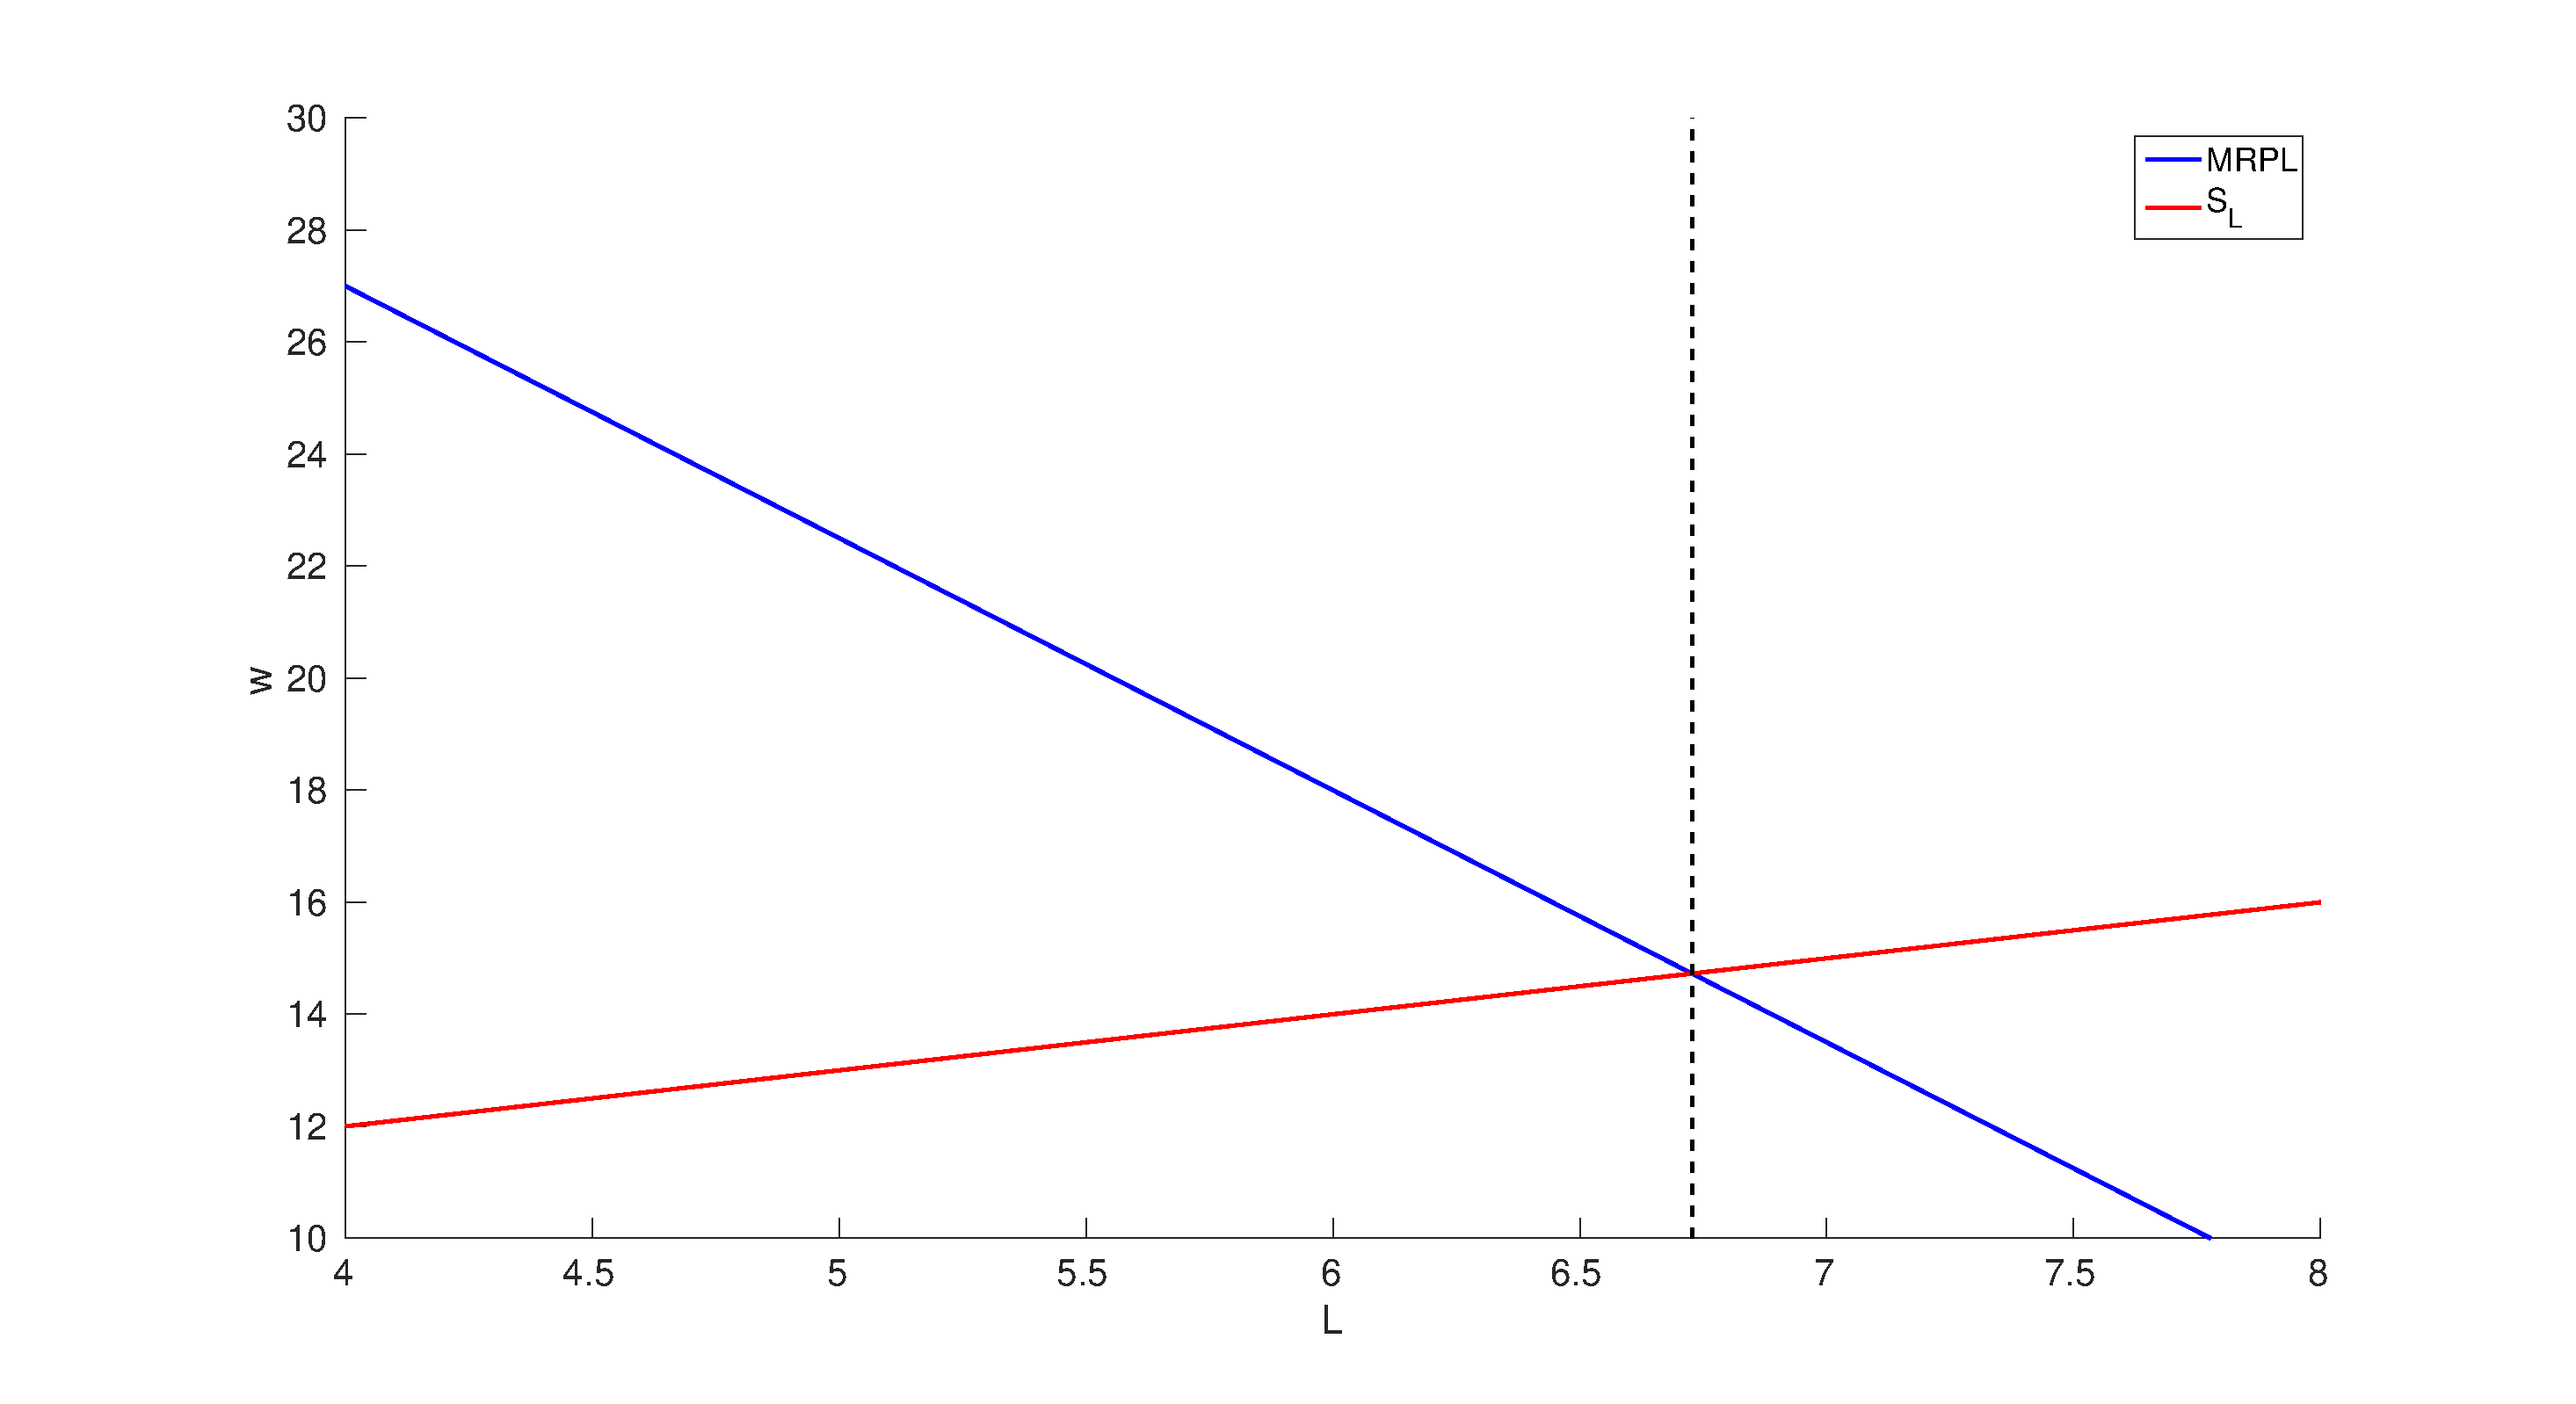
\includegraphics[width=12cm]{fig1.eps}\\
	\caption{Graphical illustration of a competitive market}\label{fig1}
\end{figure}

\subsection{Subproblem 3}
This entity does not take the nurses' wages as given because it is a monopsony. Total cost of labor is $CL=Lw=L(L+8)$. Therefore,
\begin{equation*}
	MCL=\frac{\partial(CL)}{\partial L}=2L+8
\end{equation*}

$MCL$ is upward sloping because the constant coefficient $2>0$. The general reason for $MCL$ to be upward sloping is that, the firm has to pay for the additional worker as well as pay additional wages to previously hired workers. Because of this, $MCL$ should be steeper than the labor supply curve. This is true, since
\begin{equation*}
	\frac{dw(L)}{dL}=1<\frac{d(MCL)}{dL}=2
\end{equation*}


\subsection{Subproblem 4}
In a monopsonistic market, the firm hires labor until $MRPL$ equals $MCL$.
\begin{equation*}
	MRPL=-4.5L+45=MCL=2L+8
\end{equation*}

The solution is
\begin{align*}
	&L=\frac{74}{13}\\
	&w=\frac{178}{13}
\end{align*}

Therefore, $(w^M,L^M)=(178/13,74/13)\approx(13.69,5.69)$. This is shown in Fig.\ref{fig2}.
\begin{figure}[!htbp]
	\centering
	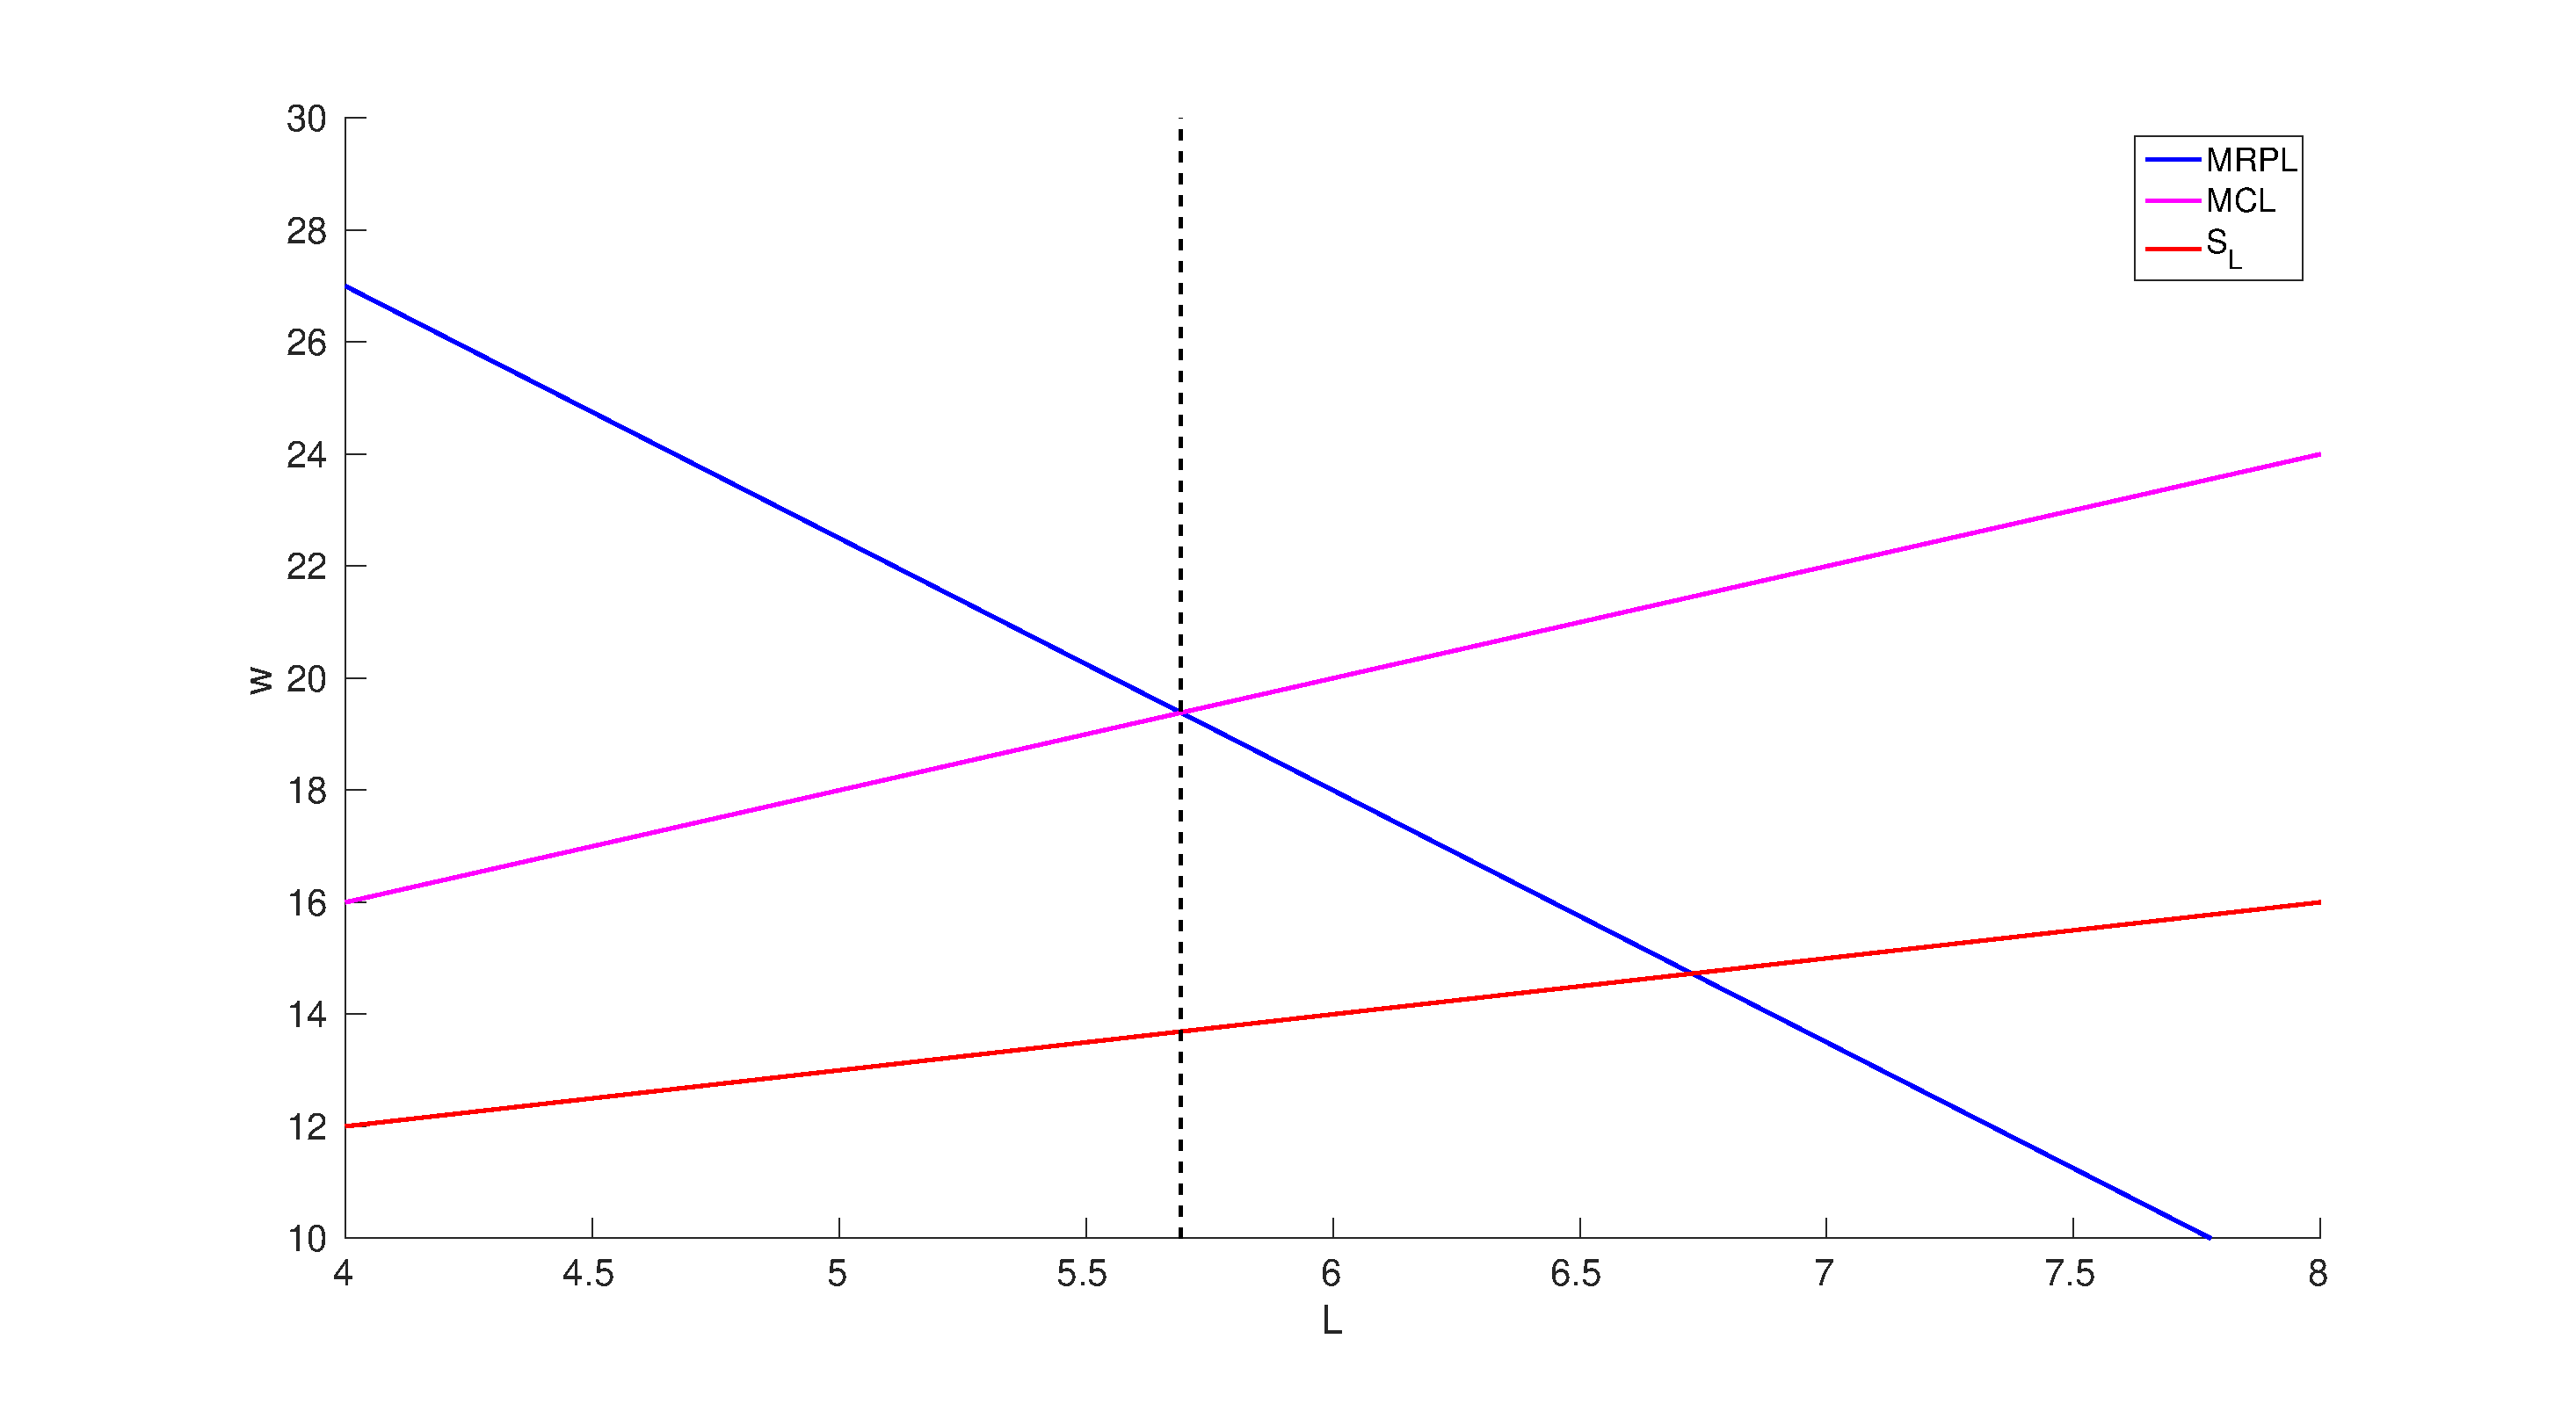
\includegraphics[width=12cm]{fig2.eps}\\
	\caption{Graphical illustration of a monopsonistic market}\label{fig2}
\end{figure}

\subsection{Subproblem 5}
The monopsonistic market has both equilibrium wage and labor lower than the competitive market. This makes sense, since the monopsony must pay additional wages to the previously hired workers when it hires someone new, it tends to hire less than in the competitive market. And a lower equilibrium labor means a lower wage in the market.

The US health care system is more like a competitive market, because there are lots of firms hiring people. Each firm is not able to hire so many workers that its hiring affects the market price of labor.

\subsection{Subproblem 6}
We notice that for both the competitive and the monopsonistic market, this minimum wage of $\$16$ is binding.

For the competitive market, the firm hires until $MRPL$ equals $w_{min}$.
\begin{equation*}
	MRPL=-4.5L+45=w_{min}=16
\end{equation*}

The new equilibrium is $(w_{min}^C,L_{min}^C)=(16,58/9)\approx(16,6.44)$. Compared with $(w^C,L^C)\approx(14.73,6.73)$, the equilibrium wage increases but the equilibrium labor drops when a minimum wage is enforced.

For the monopsonistic market, the firm is no longer a monopsony when a binding minimum wage is enforced. Then the firm just hires until $MRPL$ equals $w_{min}$, and it should reach the competitive equilibria $(w_{min}^M,L_{min}^M)=(w_{min}^C,L_{min}^C)=(16,58/9)\approx(16,6.44)$. Compared with $(w^M,L^M)\approx(13.69,5.69)$, both the equilibrium wage and labor increase. This is shown in Fig.\ref{fig3}.
\begin{figure}[!htbp]
	\centering
	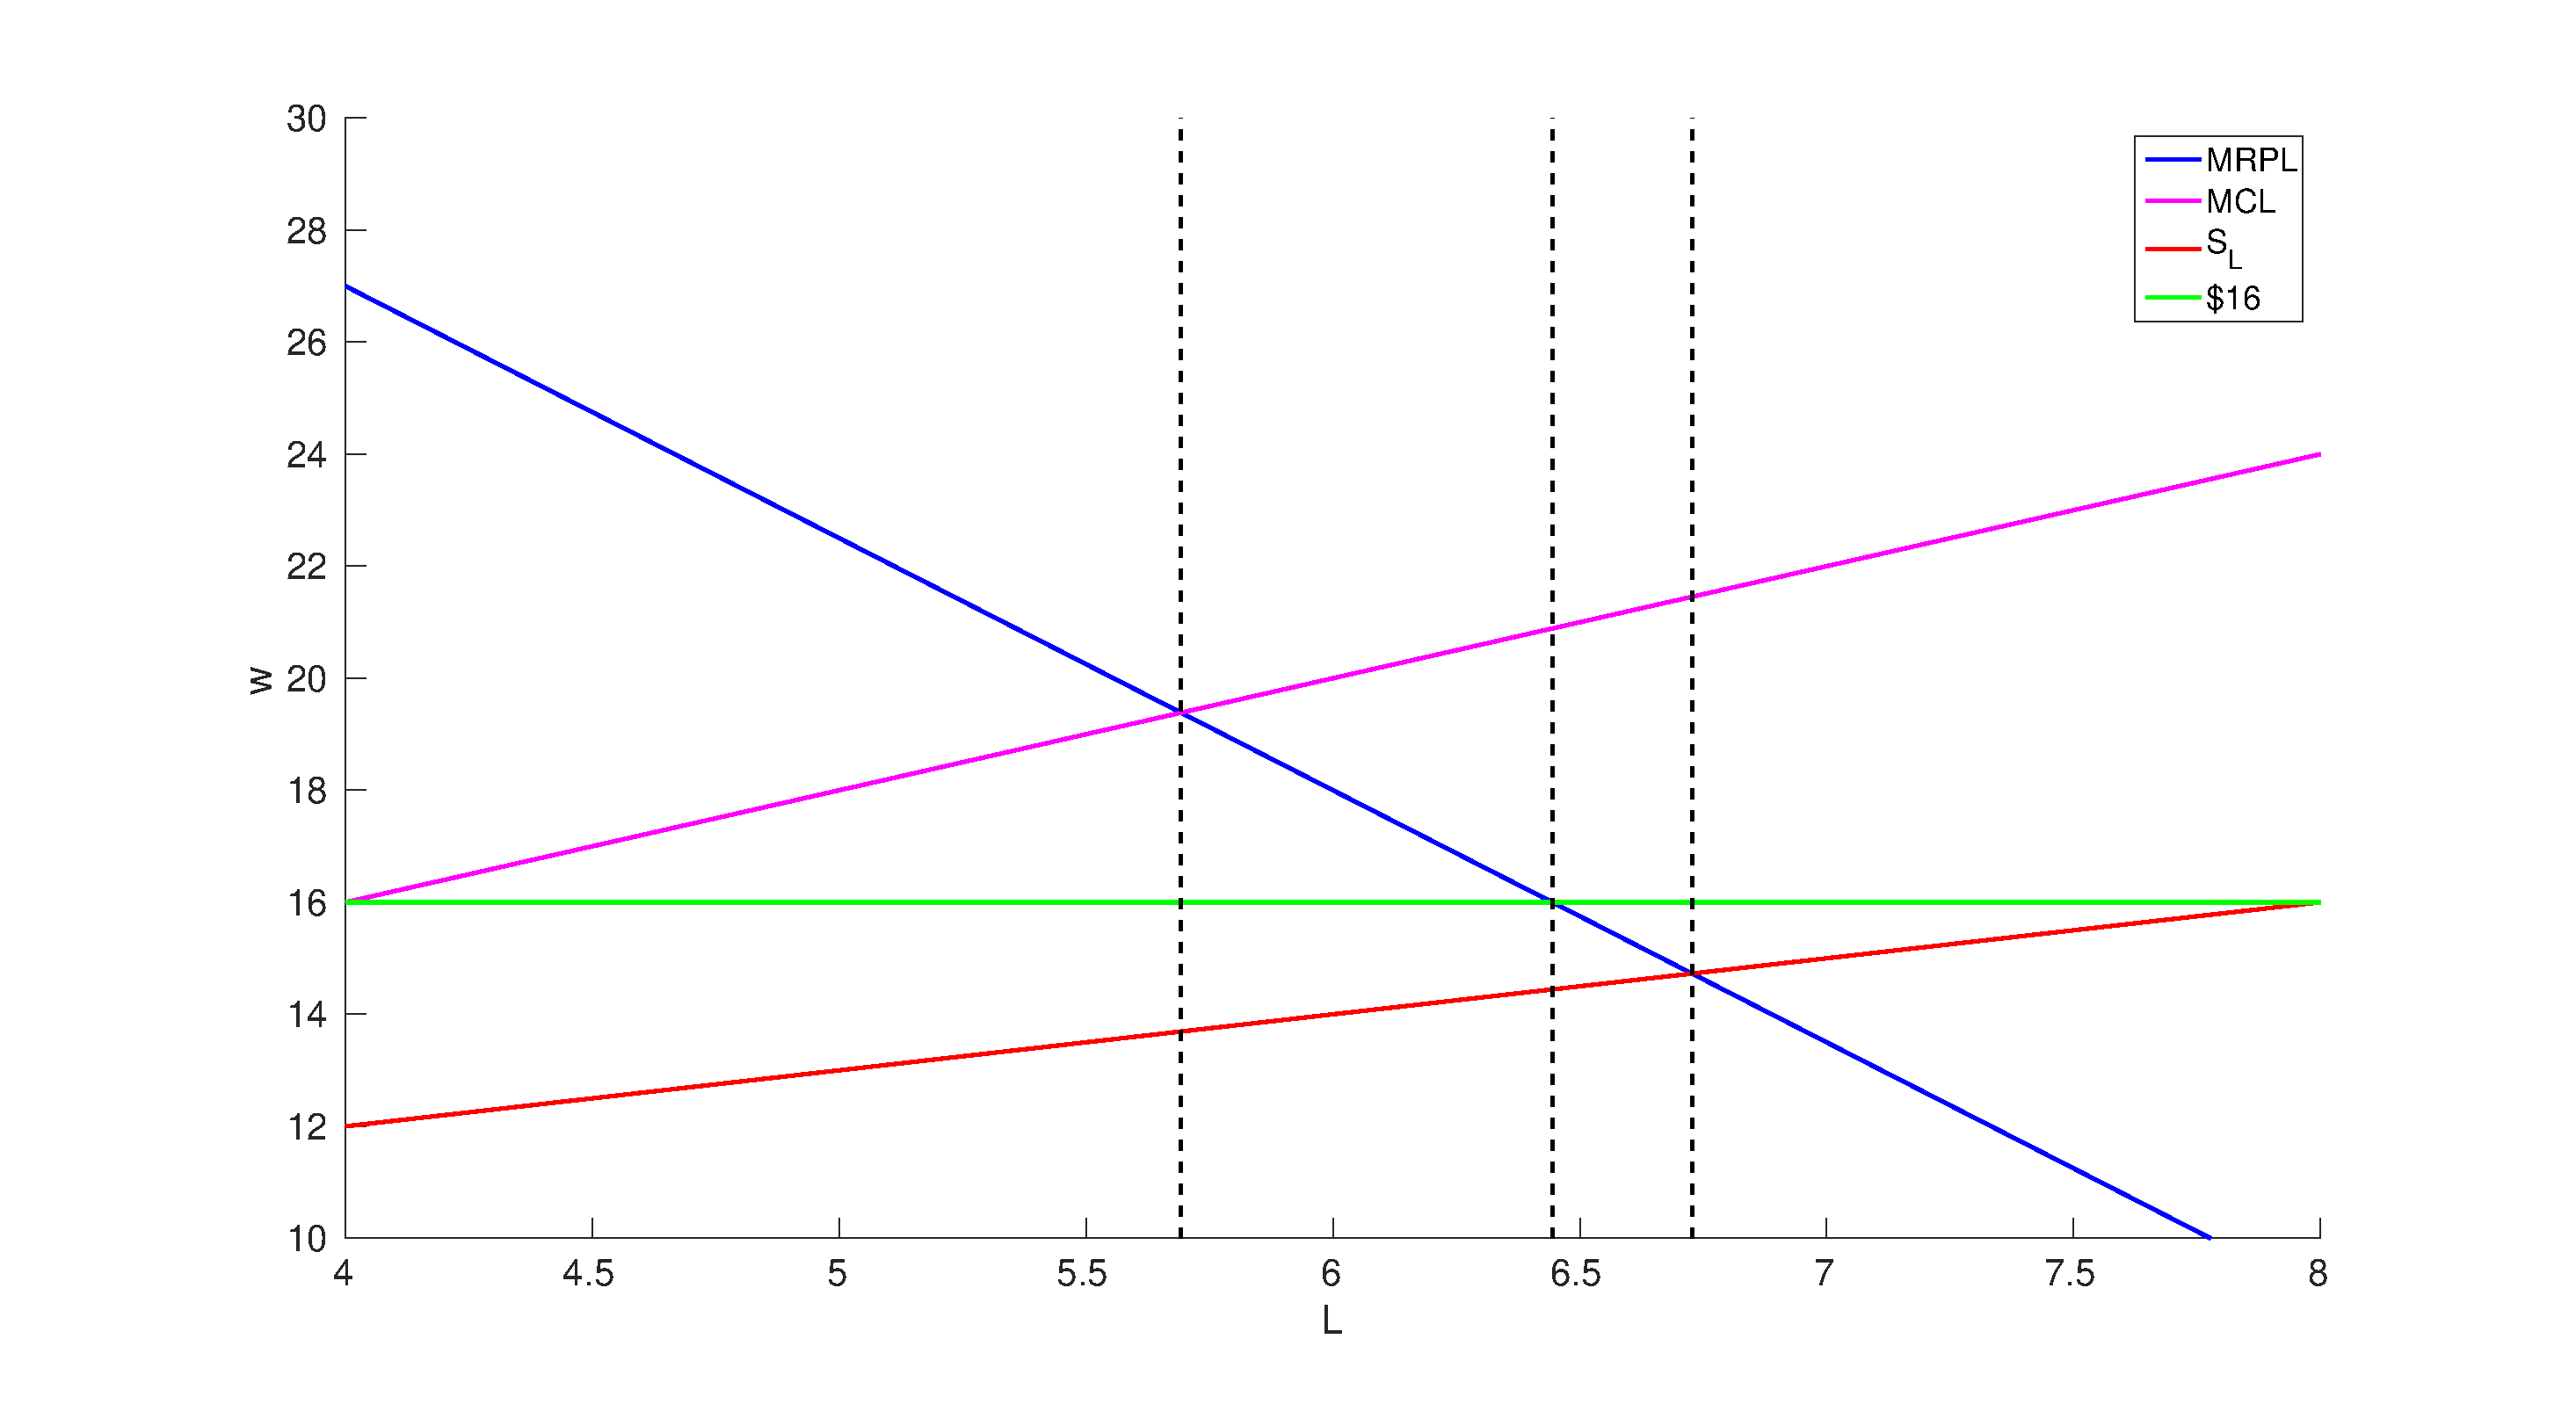
\includegraphics[width=12cm]{fig3.eps}\\
	\caption{Graphical illustration of the effect of a minimum wage}\label{fig3}
\end{figure}

\subsection{Subproblem 7}
The equation $MRPL=w_{min}=20$ has equilibrium solution $(w_{min},L_{min})=(20,50/9)\approx(20,5.56)$. As in the previous part, this solution holds not only for the competitive market, but also for the monopsonistic market, for the monopsonistic market becomes competitive under the binding minimum wage. For the competitive market, the wage increases but the labor drops. The same is true for the (previously) monopsonistic market. Notice that if $w_{min}$ is set too high, the monopsonistic market does not display an increasing equilibrium labor any more. This is shown in Fig.\ref{fig4}.
\begin{figure}[!htbp]
	\centering
	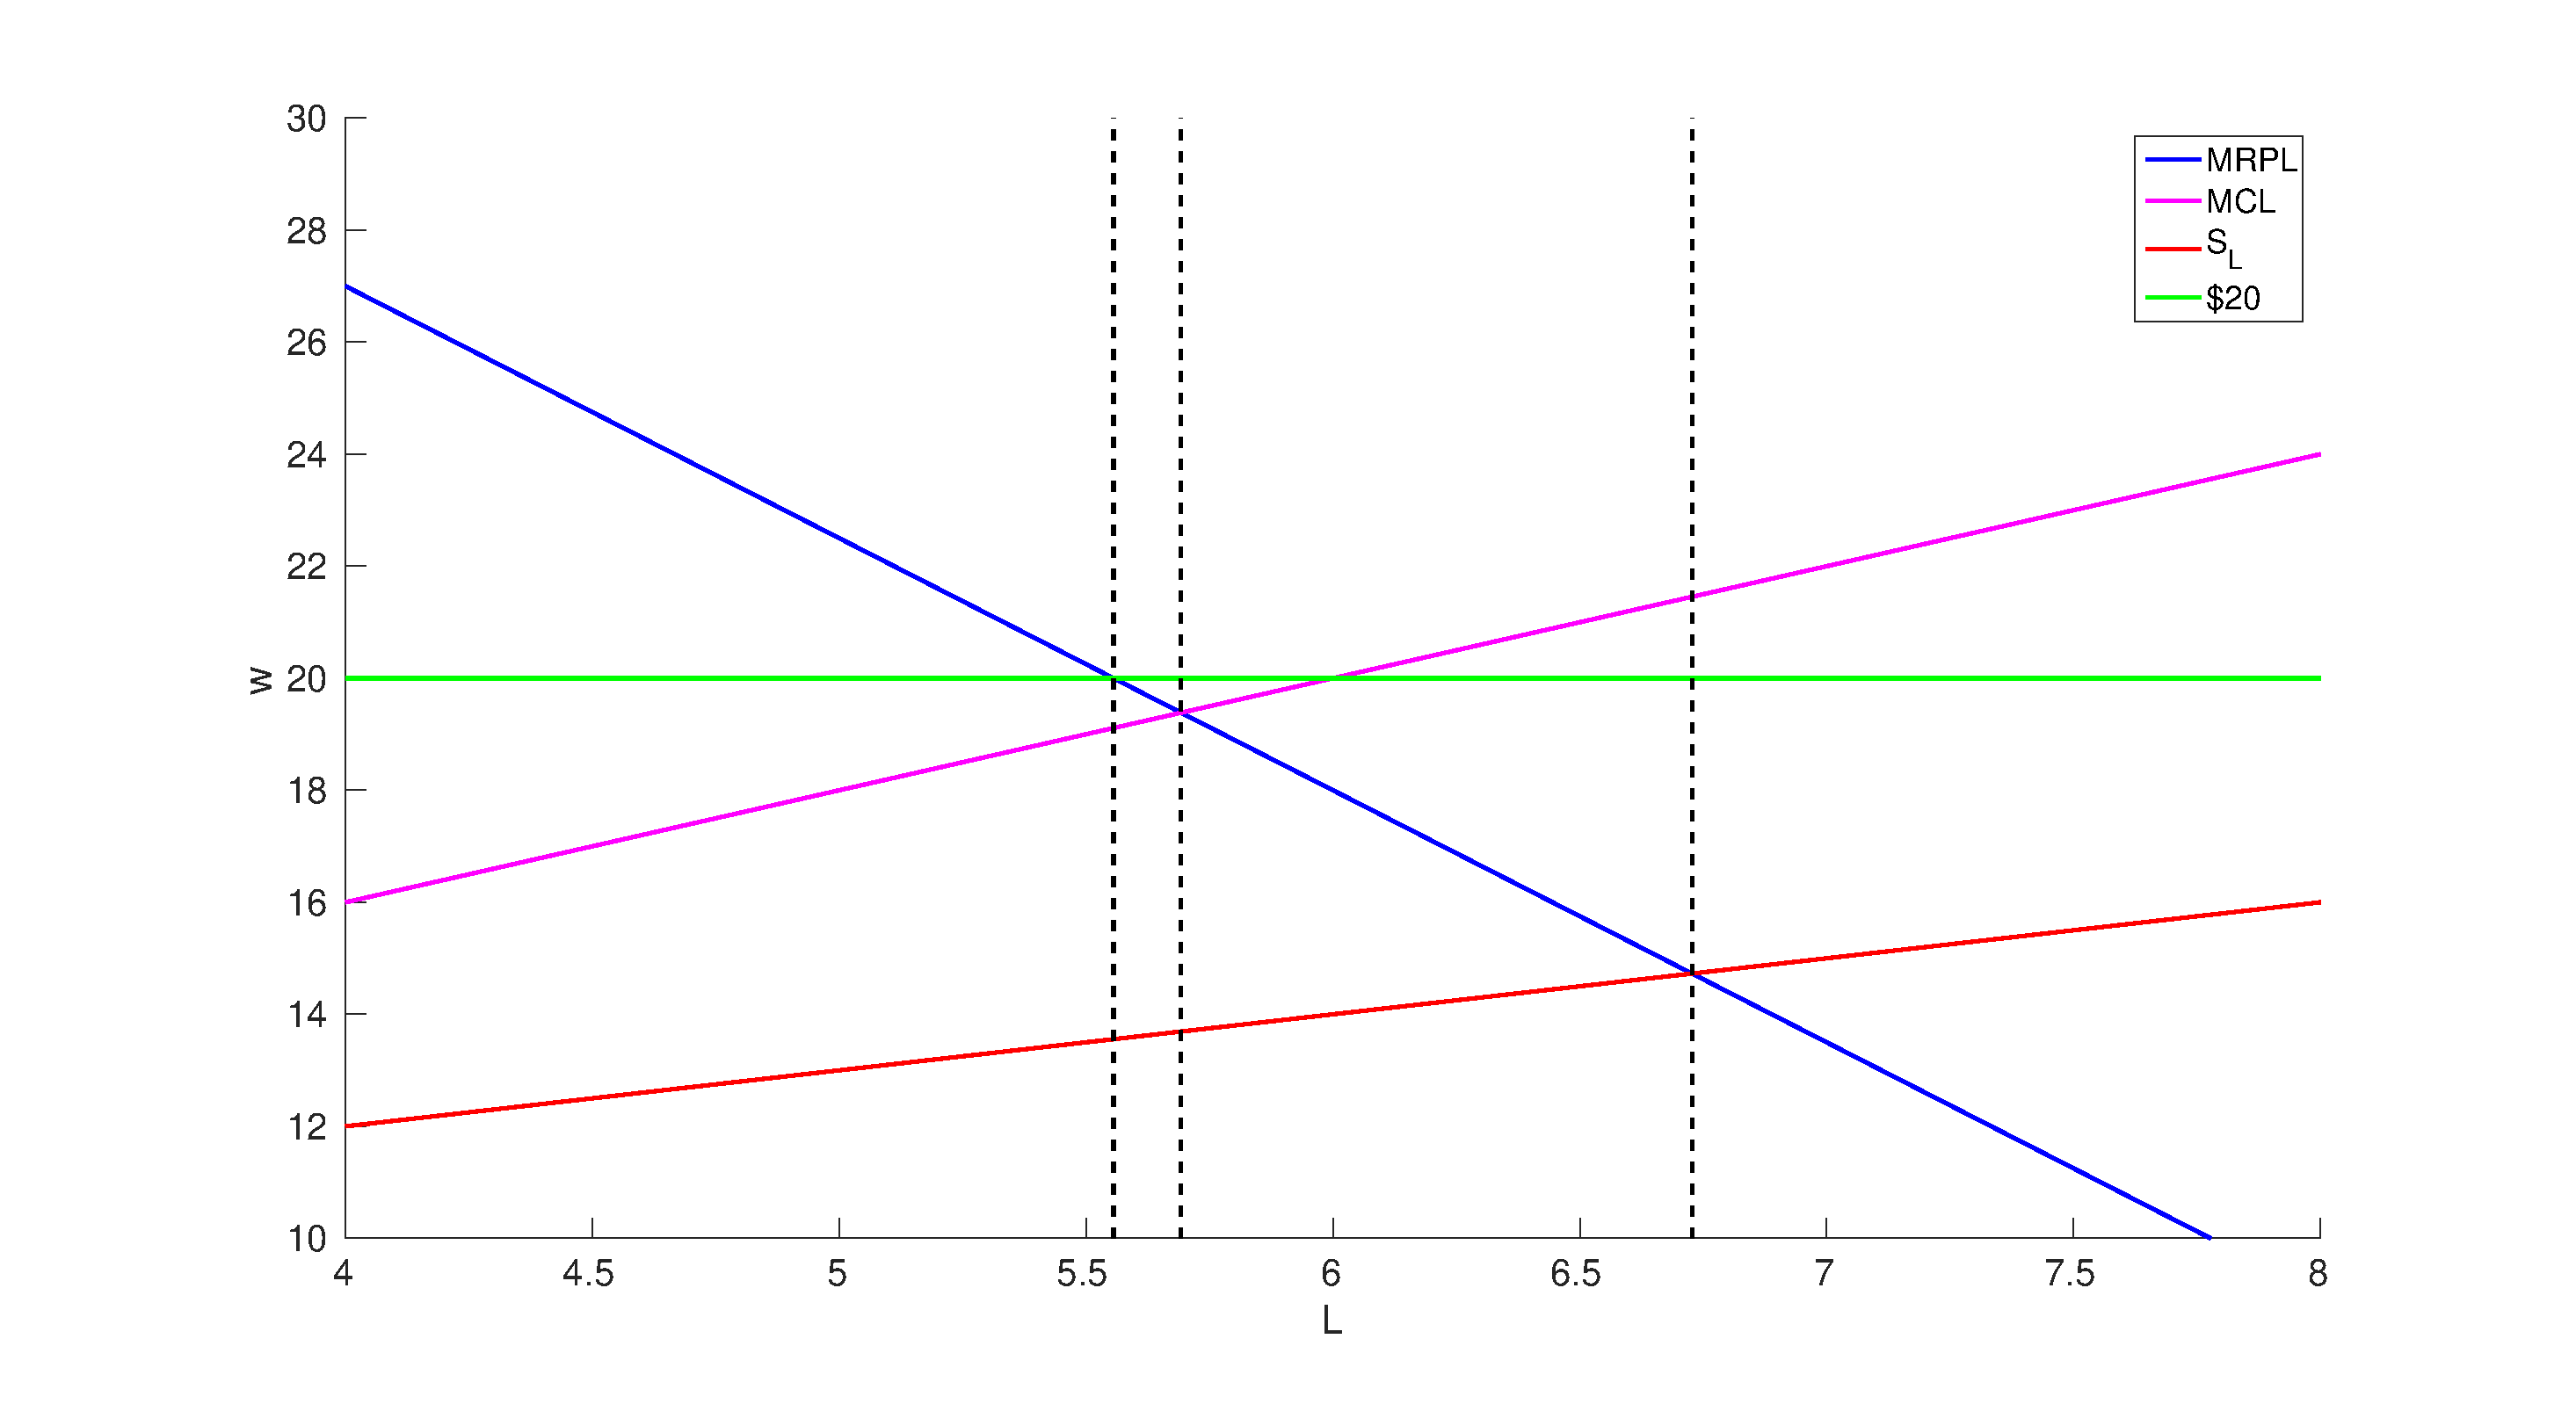
\includegraphics[width=12cm]{fig4.eps}\\
	\caption{Graphical illustration of the effect of too high a minimum wage}\label{fig4}
\end{figure}

\section{Minimum Wages and Imployment in the US}
\subsection{Subproblem 1}
The empirical results on employments suggest that the labor market can be better described as MONOPSONISTIC. This conclusion is relied on the observations that previous increase in minimum wage did not lead to decrease of employment. Examples are the early 1990s study on fast-food industry on the Pennsylvania-New Jersey border, as well as the citywide increase of minimum wage in Santa Fe. Also, the suggestion of setting different minimum wages for different areas implies that the labor is ``local'', which makes the market more monopsonistic. The uncertainty of the new \$15 minimum wage, on the other hand, can be explained by the fact that even in a monopsonistic market, too high a minimum wage can reduce employment.

\subsection{Subproblem 2}
The impact of a minimum wage will be more significant immediately before an economic boom than in a recession for a monopsonistic market. The reason is as follows.

First of all, an increase in overall economy leads to an increase in $MRPL$. This is due to the fact that business is generally better. If all other factors are fixed, then as is illustrated in Fig.\ref{CK_MRPL}, setting a minimum wage increases employment more than in a recession, where $MRPL$ is lower.
\begin{figure}[!htbp]
	\centering
	
\includegraphics[width=12cm]{blank.png}\\
	\caption{An increase in $MRPL$ leads to a more significant increase in employment}\label{CK_MRPL}
\end{figure}

Second, in an economic boom $S_L$ shifts inwards (upwards), for people are generally expecting higher wages. This also leads to an increase in $MCL$. If all other factors are fixed, then as is illustrated in Fig.\ref{CK_MCL}, setting a minimum wage still increases employment more than in a recession, where $MCL$ is lower.
\begin{figure}[!htbp]
	\centering
	
\includegraphics[width=12cm]{blank.png}\\
	\caption{An increase in $MCL$ leads to a more significant increase in employment}\label{CK_MCL}
\end{figure}

Overall, the increase in employment would be more significant if Card and Krueger did the survey immediately before an economic boom. But this effect may be more obscured by other effects that come along with the economic boom. 

\subsection{Subproblem 3}
\noindent\underline{Reason 1}: Setting a minimum wage is actually taking more money from firms and giving them to labor. This hurts the firms especially if they were labor-intensive and were previously paying below the minimum wage. Fast-food restaurants is such an example. As a result, in the long run, some restaurants may quit the market due to the higher cost of running the business. This leads to more unemployment.

\noindent\underline{Reason 2}: Labor is not the only factor in the production function. If the price of labor increases, the industry will turn more to capital, since capital can, to some extent, substitute the role of labor. This also leads to more unemployment in the long run.

\subsection{Subproblem 4}
When Texas increases its minimum wage, if we consider the labor market as monopsonistic, its equilibrium wage and employment will both increase. And more people will immigrate from Mexico to Texas for higher wages. This is shown in Fig.\ref{Texas}.
\begin{figure}[!htbp]
	\centering
	
\includegraphics[width=12cm]{blank.png}\\
	\caption{Increasing the minimum wage in Texas leads to higher employment and more immigrant in Texas}\label{Texas}
\end{figure}

On the other hand, Mexican firms are faced with a higher $MCL$. They will find it difficult to hire people at low wages because in that situation people are more willing to work in Texas. An increase in $MCL$ leads to a higher equilibrium wage but fewer job openings in Mexico. This is shown in Fig.\ref{Mexico}.
\begin{figure}[!htbp]
	\centering
	
\includegraphics[width=12cm]{blank.png}\\
	\caption{Increasing the minimum wage in Texas leads to higher wage but lower employment in Mexico}\label{Mexico}
\end{figure}

In couclusion, Texas will hire more people at a higher wage, while Mexico will hire less people at a higher wage. More immigrants will move from Mexico to Texas.

\section{Causal Inference: Gun Legislation in the US}
\subsection{Subproblem 1}
We can flip all the gun regulation laws, so that those people who, in the current reality live in a laxly regulated region (those people marked by $X=1$), are put in under a strict law, and vice versa. Then we can observe $Y_{0it}|X=1$. Since $Y_{1it}|X=1$ can be observed in the real world, we can then get ATT from $T^*=E[Y_{1it}-Y_{0it}|X=1]$.

\subsection{Subproblem 2}
The fundamental problem of causal inference is that, we can never observe $Y_{0it}$ and $Y_{1it}$ for the same $i$. In other words, for those people who live under strict gun regulation, we cannot measure what will happen if they were instead living under lax laws, and vice versa.

If I wish to answer whether strict gun regulation reduces crime, I will be interested in ATE, $T^\dag=E[Y_{1it}-Y_{0it}]$. However, due to the fundamental problem of causal inference, it is impossible to directly measure this quantity. We have to make some homogeneity assumptions and do some randomization to get ATE.

\subsection{Subproblem 3}
ATE is $T^\dag=E[Y_{1it}-Y_{0it}]$, while ATT is $T^*=E[Y_{1it}-Y_{0it}|X=1]$. The difference is that ATE reflects the expecation of the entire population, but ATT takes the expectation over only those who are treated, in other words, who are living under a strict gun control law. These two values are generally different because there might be self-selection. For example, those who are ``naturally'' more likely to commit a crime might tend to move to places that do not have strict control over guns.

The UK study gives ATT since the people are living under strict laws and thus are marked as $X=1$. This result cannot be applied to the US, for the gun law is rather lax and people here are marked as $X=0$. It is improper to use ATT to study the untreated population.

\subsection{Subproblem 4}
\subsubsection{Subsubproblem (a)}
What we can measure is $E[\hat{T}]=E[Y_{1it}|X=1]-E[Y_{0it}|X=0]$. The bias from $T^*$ can be calculated as
\begin{align*}
	Bias&=E[\hat{T}]-T^*\\
	&=E[Y_{1it}|X=1]-E[Y_{0it}|X=0]-E[Y_{1it}-Y_{0it}|X=1]\\
	&=E[Y_{0it}|X=1]-E[Y_{0it}|X=0]
\end{align*}

Therefore, the assumption to make the bias vanish is that $E[Y_{0it}|X=1]=E[Y_{0it}|X=0]$. This means that those people who live under strict laws (who are marked as $X=1$) would make the same decision as the untreated people (who are marked as $X=0$), if they were living under lax laws. In other words, that if those British were living in the US in 1998, they would make the same expected decision as the Americans do.

\subsubsection{Subsubproblem (b)}
The assumption is not likely to be satisfied. This is because there is potential self-selection involved. If people who are ``naturally'' more likely to coommit a crime tend to live under lax gun laws, then the result can be biased.

\subsubsection{Subsubproblem (c)}
If self-selection exists, then $E[Y_{0it}|X=1]<E[Y_{0it}|X=0]$. Therefore, the bias is negative. A downward biased estimate means that $E[\hat{T}]<T^*$.

\subsection{Subproblem 5}
\subsubsection{Subsubproblem (a)}
What we can measure is $E[\hat{T}]=E[Y_{1i,1998}|X_{1998}=1]-E[Y_{0i,1996}|X_{1998}=1]$. The bias from $T^*=E[Y_{1i,1998}|X_{1998}=1]-E[Y_{0i,1998}|X_{1998}=1]$ can be calculated as
\begin{align*}
	Bias&=E[\hat{T}]-T^*\\
	&=(E[Y_{1i,1998}|X_{1998}=1]-E[Y_{0i,1996}|X_{1998}=1])-(E[Y_{1i,1998}|X_{1998}=1]-E[Y_{0i,1998}|X_{1998}=1])\\
	&=E[Y_{0i,1998}|X_{1998}=1]-E[Y_{0i,1996}|X_{1998}=1]\\
\end{align*}

Therefore, the assumption to make the bias vanish is that $E[Y_{0i,1998}|X_{1998}=1]=E[Y_{0i,1996}|X_{1998}=1]$. This means that for those living under a strict law, the decision that they would make if the law were lax is not affected by the change of time.

\subsubsection{Subsubproblem (b)}
The assumption is likely to be satisfied since the population has not changed. Both terms in the bias are relative to the treated people. It is likely that there is not much time effect.

\subsubsection{Subsubproblem (c)}
The sign of the bias cannot be determined, since it is hard to deduce the time effect on the population.

\subsection{Subproblem 6}
From part 4, we get $Y_{UK,1998}-Y_{US,1998}$. From part 5, we get $Y_{UK,1998}-Y_{UK,1996}$. In order to calculate DID, we also need $Y_{US,1996}$. Then we have
\begin{align*}
	DID=&E[\Delta Y_{UK}-\Delta Y_{US}]\\
	=&(E[Y_{1i,1998}|X=1]-E[Y_{0i,1996}|X=1])-(E[Y_{0i,1998}|X=0]-E[Y_{0i,1996}|X=0])\\
	=&(E[Y_{1i,1998}|X=1]-E[Y_{0i,1998}|X=1])+(E[Y_{0i,1998}|X=1]-E[Y_{0i,1996}|X=1])-\\
	&(E[Y_{0i,1998}|X=0]-E[Y_{0i,1996}|X=0])\\
	=&T^*+TE_{UK}-TE_{US}
\end{align*}
where $TE$ stands for time effect.

In order for DID to reflect $T^*$, we must assume that the time effect for the UK and the US are about the same, so they cancel out and only $T^*$ survives.

\subsection{Subproblem 7}
From the graph, we can estimate $Y_{UK,1996},Y_{UK,1998},Y_{US,1996}$ and $Y_{US,1998}$ which, by calculation, gives a positive DID. This means that, according to the calculation, a stricter gun legislation is accompanied with a upward ATT. However, this does not necessarily mean that gun legislation is responsible for the increase in crime. It is very likely that there are other effects, for example an increase of unemployment, that is causing the rise of crime rate. And legislation is possibly only a governmental response to this exogenous risk of crime increase.

This exogenous reason affects my estimated $T^*$ by making it more positive. Intuitively, we would expect $T^*<0$. But as is shown in the figure, this effect flips the sign of $T^*$. This is especially true if we notice the sharp increase in the rate of crime after 1998, where our conclusion can be greatly mislead.

\end{document}
